\documentclass{article}
\usepackage[T1]{fontenc}
\usepackage[english]{babel}
\usepackage{csquotes}
\usepackage{amsmath}
\usepackage{graphicx}
\usepackage{booktabs}
\usepackage[style=authoryear]{biblatex}
\addbibresource{references.bib}
\usepackage[colorlinks=true, allcolors=blue]{hyperref}

\title{{{TITLE}}}
\author{{{AUTHOR}}}
\date{\today}

\begin{document}

\maketitle

\begin{abstract}
This example project shows, in a few pages, what is most often written with
\LaTeX{}: sections, a figure, a table, lists, mathematics and references.
Change it as you like.
\end{abstract}

\section{Getting started}

The \LaTeX{} code is on the left and the PDF on the right. To update the PDF,
click the compile button or press Ctrl+Enter (Cmd+Enter on a Mac).
Double-clicking in the PDF takes you to the matching line of code.

\subsection{Sections and subsections}

The \verb|\section| and \verb|\subsection| commands divide the text. They are
numbered automatically, and \verb|\tableofcontents| turns them into a table
of contents.

\section{Figures}

Figure~\ref{fig:curves} shows the project's image \texttt{images/curves.png}.
To add your own, upload them to the \texttt{images} folder or use the
\enquote{Insert figure} button of the toolbar.

\begin{figure}[htbp]
  \centering
  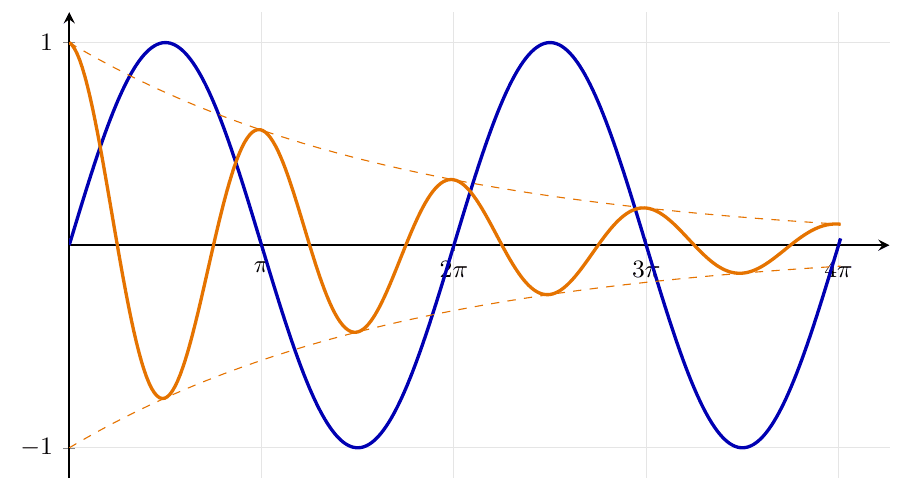
\includegraphics[width=0.8\linewidth]{images/curves.png}
  \caption{A sine wave and a damped oscillation.}
  \label{fig:curves}
\end{figure}

\section{Tables}

Table~\ref{tab:measurements} uses the rules of the \texttt{booktabs}
package.

\begin{table}[htbp]
  \centering
  \caption{A few measurements.}
  \label{tab:measurements}
  \begin{tabular}{lrr}
    \toprule
    Trial & Duration (s) & Temperature (°C) \\
    \midrule
    A & 12.5 & 21.3 \\
    B & 14.1 & 22.8 \\
    C & 11.9 & 20.6 \\
    \bottomrule
  \end{tabular}
\end{table}

\section{Lists}

A bulleted list:
\begin{itemize}
  \item items in no particular order,
  \item set out by the \texttt{itemize} environment.
\end{itemize}
A numbered list:
\begin{enumerate}
  \item a first step,
  \item then a second one, with \texttt{enumerate}.
\end{enumerate}

\section{Mathematics}

Formulas are written within the text, between dollar signs, as $E = mc^2$,
or centred and numbered:
\begin{equation}
  \int_0^{\infty} e^{-x^2} \, \mathrm{d}x = \frac{\sqrt{\pi}}{2}.
  \label{eq:gauss}
\end{equation}
Equation~\eqref{eq:gauss} is the Gaussian integral. The \texttt{align}
environment aligns several lines:
\begin{align}
  (a + b)^2 &= a^2 + 2ab + b^2, \\
  (a + b)(a - b) &= a^2 - b^2.
\end{align}

\section{Margins and paper size}

The \texttt{geometry} package sets the paper size and the margins. For
example, in the preamble:
\begin{verbatim}
\usepackage[letterpaper, margin=1in]{geometry}
\end{verbatim}
Replace \texttt{letterpaper} with \texttt{a4paper} for A4 paper.

\section{References}

The references are in \texttt{references.bib}. They are cited with
\verb|\textcite| or \verb|\parencite|: \textcite{knuth1984} created \TeX{},
then \textcite{lamport1994} wrote \LaTeX{} on top of it. The bibliography is
set at the end of the document on its own \parencite{mittelbach2023}.

\printbibliography

\end{document}
